\chapter{Background}
\label{background}

We begin this section by describing a \ac{CPS} attack in terms of three parties involved; this decomposition will lead into our attack model in Chapter~\ref{attack}.
Next, we provide a summary of canonical \ac{CPS} so we can then introduce conventional controller designs and its limitations. 
We then define \ac{DNN} based models and describe the open problems in them. 
Finally, we conclude the section with a formal problem statement. 


\section{Roles description}
There are three parties involved in designing and attacking \ac{CPS}. These are important to identify the different pieces of information an attacker needs to gather to attack a system.

\begin{enumerate}
	\item \textbf{Specification Designer/Domain Expert:} The domain expert is responsible for developing the system specification. 
	For an \ac{APS}, the domain expert specifies the safe thresholds for the amount of insulin injected into a patient. The domain expert also indicates values that should trigger alarms, e.g., in case of a high blood glucose reading.
	\item \textbf{System Developer:} These are the people who build the controller models, e.g., a decision trees, \ac{DNN} or a conventional controller model to implement the system.
	\item \textbf{Attacker:} The attacker is trying to make the system misbehave by injecting false sensor readings in the \ac{CPS} without triggering safety alarms specified by the domain expert . 
\end{enumerate}

\begin{figure}
	\centering
	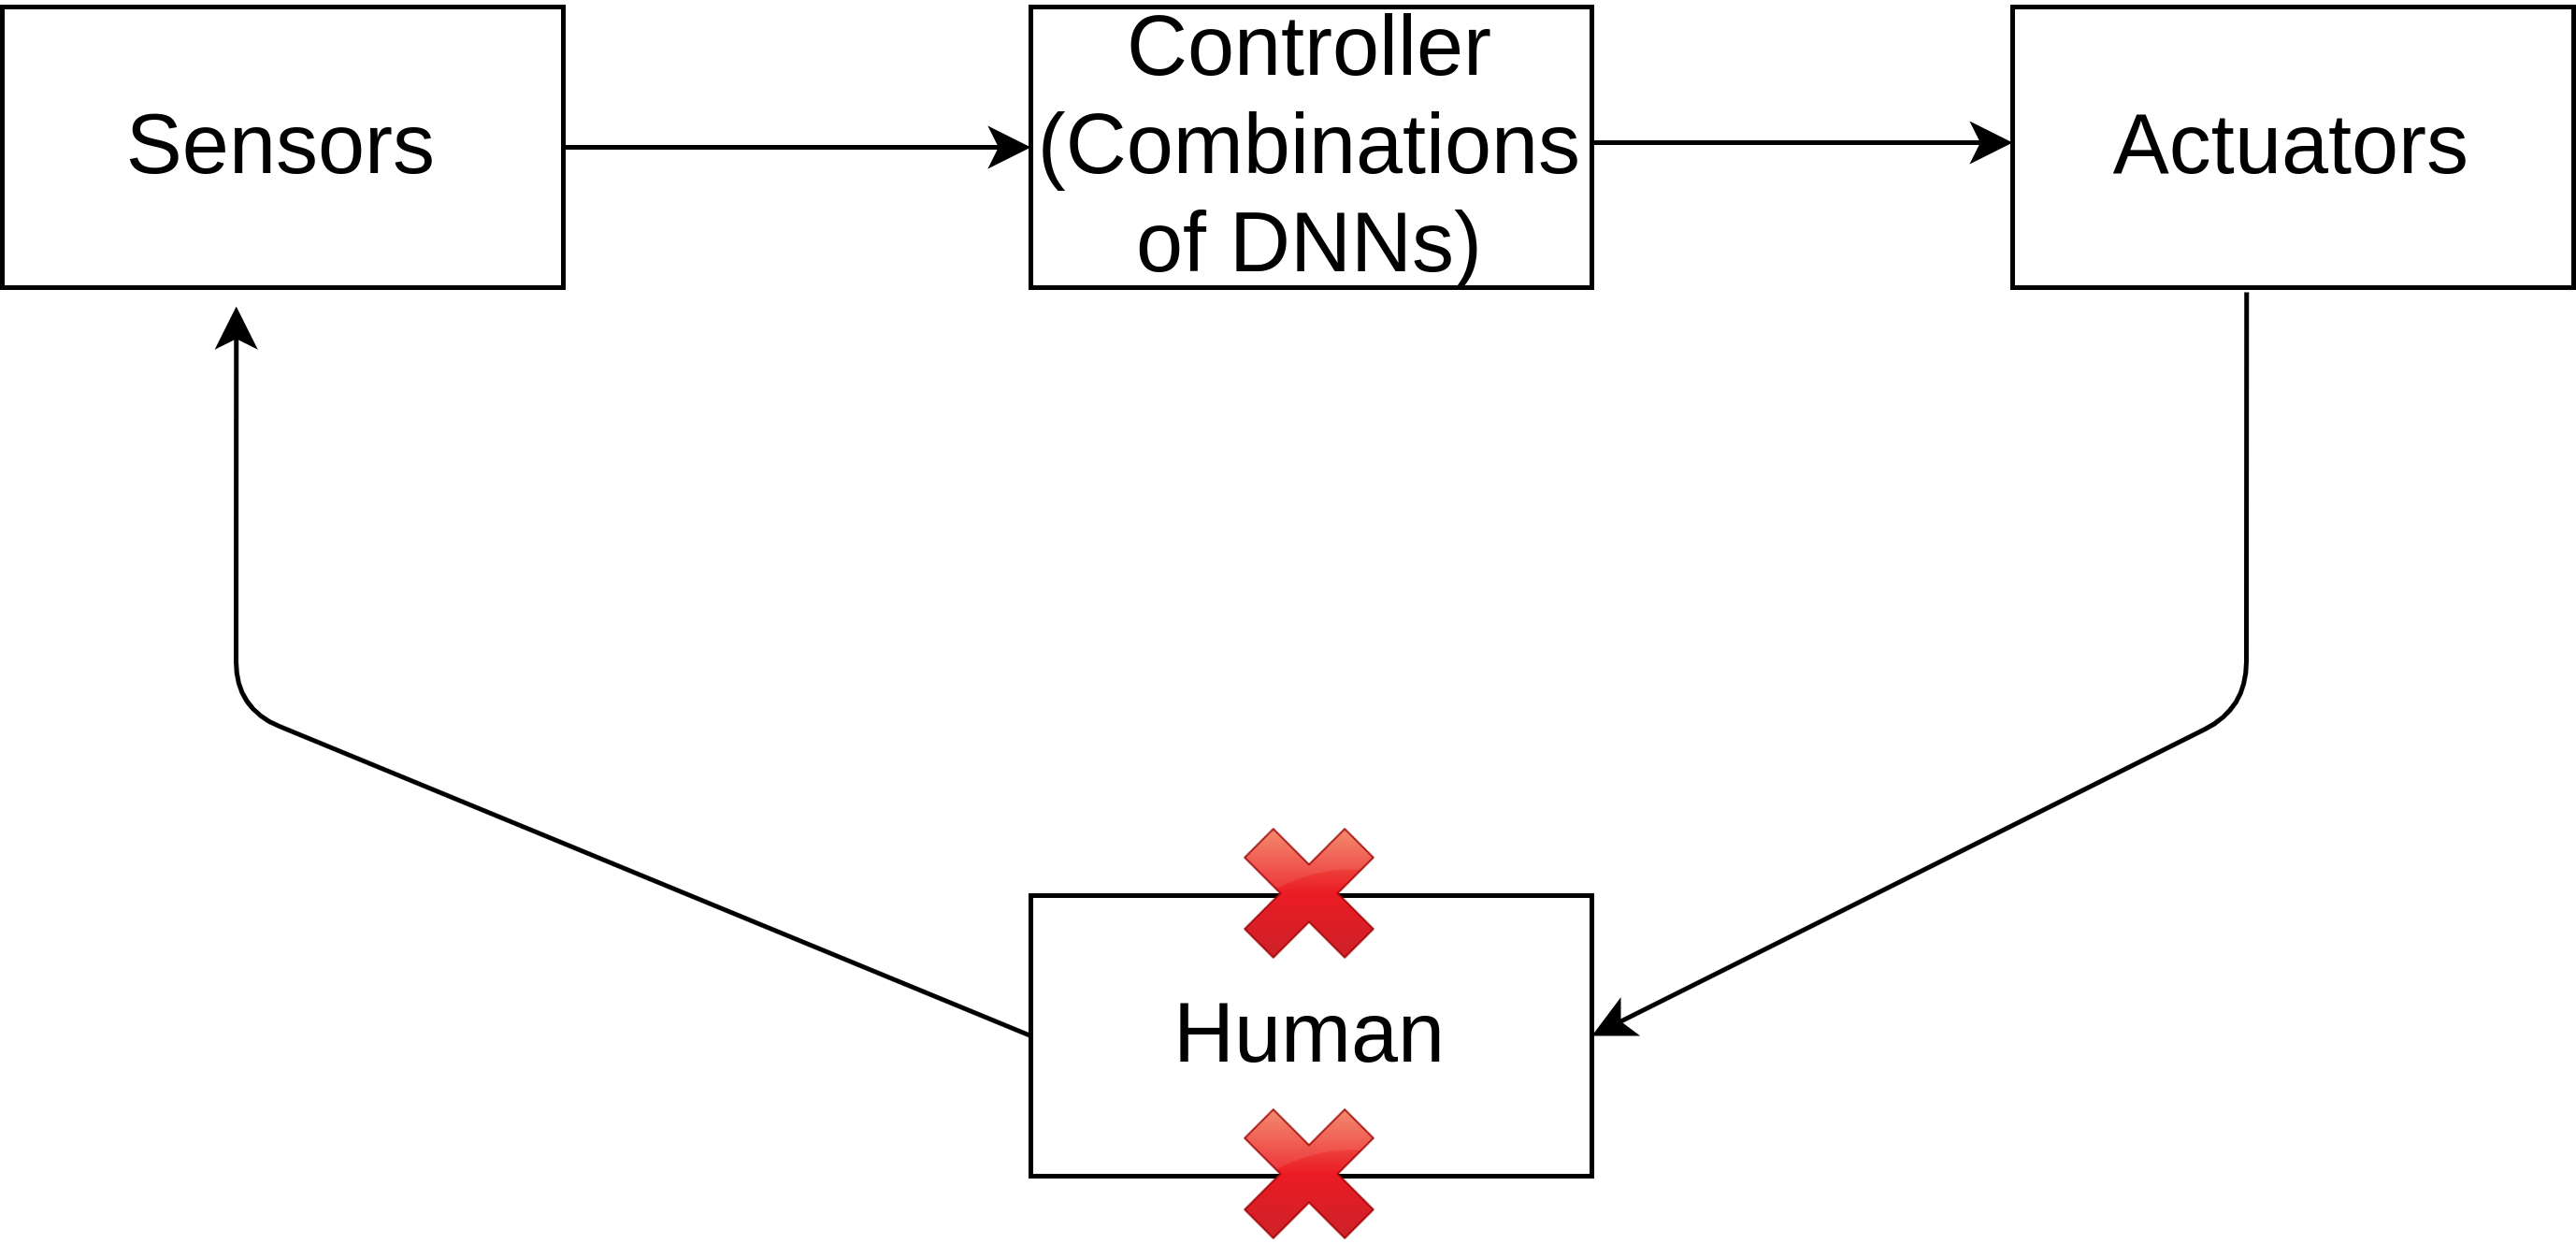
\includegraphics[width=0.7\linewidth]{Images/Systemsdescription}
	\caption{Architecture of a CPS}
	\label{fig:systemsdescription}
\end{figure}

\begin{figure}
	\centering
	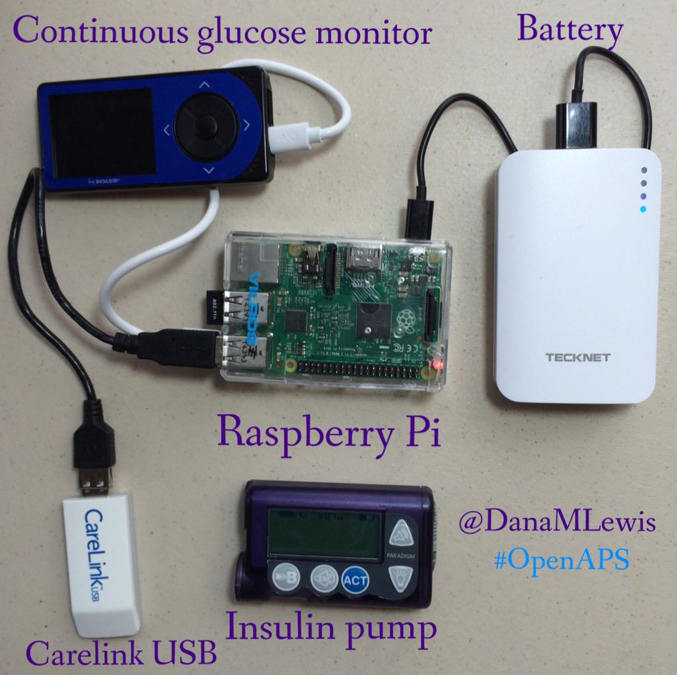
\includegraphics[width=0.7\linewidth]{Images/APSrig}
	\caption{Artifical Pancreas System components \\
		Source: www.openAPS.org}
	\label{fig:apsrig}
\end{figure}



\begin{figure}
	\centering
	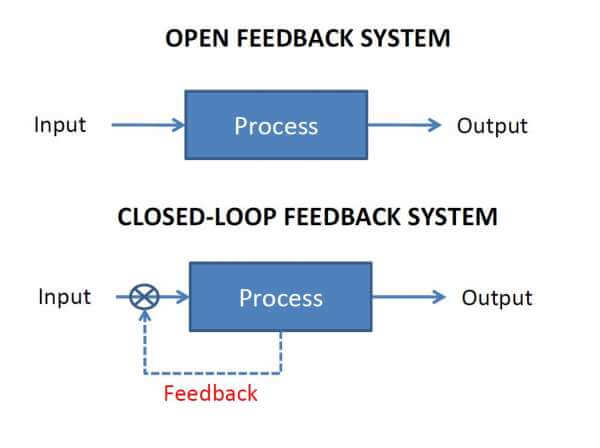
\includegraphics[width=0.7\linewidth]{Images/closedvsopen}
	\caption{General structure of a open and closed-loop systems 
		Source:https://instrumentationtools.com/open-loop-and-closed-loop-animation/ }
	\label{fig:closedvsopen}
\end{figure}


\section{Cyber-Physical Systems}
\ac{CPS} are systems that use sensor readings from the physical world to perform computations that produce changes in the physical  world.   
As shown in Figure ~\ref{fig:systemsdescription}, the sensors and actuators are the physical parts of the system. 
The sensors gather data from the physical environment and send it to the computational unit. 
The computational unit is a controller, which makes decisions that are sent to the actuator, which in turn  physically performs the action.
The physical and virtual contexts can either be humans in the loop or automated mechanisms.

In the \ac{APS} shown in Figure ~\ref{fig:apsrig}, the sensor is the \ac{CGM} that is attached to the back of a patient to report blood glucose level.  
\ac{RPi} is the computational part of the \ac{APS}, and the insulin pump is the actuator. 

There are two types of CPS: open feedback and closed-loop feedback.
In open feedback systems, 
%there is human intervention during the decision making process. 
as shown in Figure ~\ref{fig:closedvsopen} (top), the human is a part of the loop; he/she keeps track of the decisions being taken by the controller. 
In closed-loop systems, there is no human intervention 
as shown in Figure ~\ref{fig:closedvsopen} (bottom). 
In the latter case, understanding different types of security attacks becomes a necessity, because automation means that once the attacker has found a way to tamper with the automation mechanism, they can break the system. 
In the case of stealthy (or subtle) attacks, as will be described in Chapter ~\ref{attack}, 
closed loop systems are more vulnerable because existing error-detection mechanisms can be reverse engineered and then used to attack the systems. 

\section{Conventional Controllers for CPS}

A conventional controller transforms into decisions the sensors readings using sets of differential equations for the controller. 
For instance, a quadcopter contains multiple flight modes in its controller based on the weather conditions such as windy or normal day. 
These modes are important because during windy weather, the decision making model for stable quadcopter flights will be different from a normal weather flight \cite{inbook}. 

Based on the inputs or data collected from the sensors, the appropriate  mode is selected and the decision is calculated. 
Every mode consists of a different set of equations, because every mode represents a different scenario.
Figure ~\ref{fig:controltheory} shows a position control system of a quadcopter \cite{inbook}. The input values use the derived version of the equations that are used in decision making. 

\begin{figure}
	\centering
	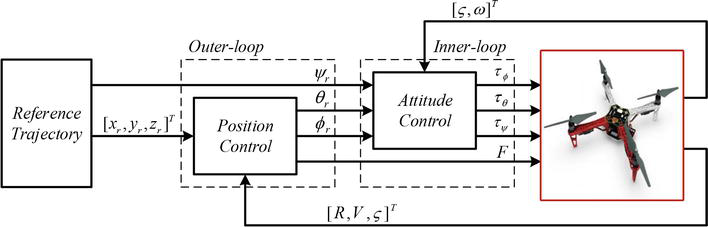
\includegraphics[width=0.7\linewidth]{Images/controltheory}
	\caption{The block diagram of the position control system of the quadcopter.
	}
	\label{fig:controltheory} 
\end{figure}


%How are they modeled
These modes use classical control theory that is represented as a set of equations designed by domain experts.
For instance, the model for a medical system such as \ac{APS} can be designed only if the specifications are known for the medical system. 
A part of the specification such as the important parameters (insulin, blood glucose etc. in APS) and their threshold values are provided by domain (in this case medical) experts. 
Another important aspect for designing control systems is modeling the precise relations between the parameters. 
This is possible in systems such as APS, because it is a simpler system compared to self-driving car. 
However, designing the precise mathematical relations for systems such as self-driving cars can be tedious \cite{article23}, as we elaborate below.

The move from equation-based models to DNNs for modeling \ac{CPS} behavior has been justified by the following observations:
\begin{enumerate}
	\item CPS behavior is controlled using a lot of input data from the many sensors a system might have. The self-learning nature of DNNs lends itself well to model behavior driven by sensor input. This is easier than formulating the control theoretic differential equations, which need domain and mathematical expertise \cite{Aamir_2013}.
	
	
	To look at a more concrete example, consider a medical system such as \ac{APS}, which uses conventional control theory to build models. 
	Forming the model requires the programmer to be aware of not only the intended system behavior and the mathematical formulation needed to produce the desired result. 
	DNNs, on the other hand, can automatically build models given data.
	Training DNNs is implicitly dependent on the quality of available training data, and it is a known problem in the field \cite{jabbar2015methods}. It does not, however, require the system designers to model precise control equations as does control theory.
	\item  There are limitations on the behaviors that can be modeled using the standard control-theoretic approaches. They do not, for instance, work well for building dynamic models \cite{article23}. Building such dynamic models is important in many systems such as in autonomous vehicles, which are essentially composed of multiple interacting control systems. Conventional control systems are not designed to work in an interactive, plug-and-play manner with other control systems, because they are built to model only one behavior. DNNs do provide this dynamic capability \cite{article23}. 
	Due to data driven modeling, it is relatively easier to build models for autonomous vehicles that have multiple models interacting within them.
	For instance, they contain separate models for image recognition and lane detection that continuously interact with each other to decide the next best course of action.
	
	\item Sarabakha et al. \cite{sarabakha2019online} show that using a \ac{DNN} based controller for a quadcopter leads to better decision making in unspecified cases compared to control theory models.
	This is due to the \ac{DNN}'s ability to adapt to different situations in contrast to the fixed nature of conventional control theory. 
	Hence, in cases when the trajectories or situations cannot be precisely modeled, the \ac{DNN} is likely to be more effective. 
\end{enumerate}




\section{DNN Based Controller}
\label{apsdnn}


%A \ac{NN} is an algorithm that is modeled after the human brain.
A \ac{NN} consists of input, output and hidden layers. 
The layers are composed of nodes. Every computation occurs within in a node of a network.
In the simplest case, there is a single neuron that takes all the inputs to produce an output, as shown in Figure 2.5. 
All inputs to the node in Figure 2.5 are summed and  passed through an activation function. 
Activation function decides, whether a neuron should be activated or not by calculating weighted sum and further adding bias with it. The purpose of the activation function is to introduce non-linearity into the output of a neuron.
A common activation function is the \ac{ReLU} function. 
The node determines up to what extent the signal must progress to calculate the final output. 
The final output depends on the network and can be in binary form or have a precise value associated with it. 


A \ac{DNN} consists of multiple hidden layers as shown in Figure 2.7, which is an example of a feed-forward \ac{DNN}, which is the simplest type of artificial neural network \cite{feedforward}.
The information flows only forward from input through layer to outputs \cite{Zell}. 

The classical controller model is being replaced by such DNN based controllers for CPS as shown in  Figure 2.6.
The \ac{DNN} for \ac*{CPS} is trained using the data gathered from conventional control equations. 
One example is the DNN based controller designed by Dutta et al. \cite{Dutta_Others__2018__Robust}. 
Dutta et al. model a robust DNN using available patient data to predict the output for an insulin pump.
Their controller design is for providing a data-driven approach for an artificial pancreas system (APS), which is also our first system used for evaluation. 

We evaluate two other systems called \ac{CA} systems for unmanned vehicles \cite{7778055} called \ac{HCAS} and \ac{ACAS-Xu}: both \ac{CA} systems are bigger in size (number of nodes and layers) and have a complex architecture in as compared to \ac{APS}.


%Normalization layers in DNN
\ac{DNN}s also consist of a feature called normalization in their layers.  
Normalization is a common feature engineering method where all the inputs are brought to standard scale since different set of inputs can be in different ranges. 
This is important in \ac{DNN}s for reasons explained by  LeCun et al.  \cite{10.5555/645754.668382}.
%The first reason is trivial as computations on a bounded range of numbers prevent some numerical inaccuracies and limit the computational power required. The second reason is that some machine learning algorithms can handle that data better when it is normalized. There are several approaches to normalization of the data.
Our two evaluation systems are aircraft  control management systems \cite{10.1007/978-3-319-63387-9_5} consist of a normalization layer, 
which we consider during our \ac{MILP} formulation in Chapter ~\ref{relusyn}.

\subsection{Understanding DNN complexity}
\label{dnncomplexity}
To understand the complexity of \ac{DNN}s we use two criteria
\begin{enumerate}
	\item Size: The size depends on two aspects, the number of layers in a \ac{DNN} and the number of nodes in each layer. 
    An increase in the hidden layers corresponds to more connections and opacity between the inputs and the outputs. 
    The increase in the number of nodes per layer corresponds to more connections between each layer which ultimately increases the input and output mapping. 
	\item Architecture: The architecture consists of the the design of the network which consists of 
	\begin{enumerate}
		\item Connectivity: For a fully-connected network, every node is connected to every node in the network.
		There are multiple different ways architectures can be designed. 
		\item Activation functions: These introduce non-linearity to the layers and have multiple different characteristics. Some networks also consist of layers that perform max/average pooling operations. 
	\end{enumerate}
	

	
\end{enumerate}
When we refer to \ac{DNN} complexity in this thesis, we are referring to differences in size and architecture.


\begin{figure}
	\centering
	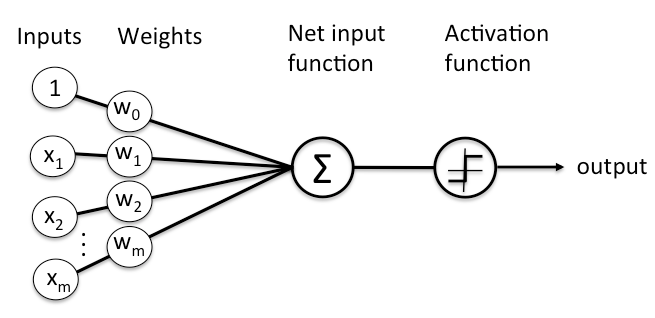
\includegraphics[width=0.7\linewidth]{Images/perceptron_node}
	\caption{Perceptron node  \\ Source: https://pathmind.com/wiki/neural-network}
	\label{fig:perceptronnode}
\end{figure}

\begin{figure}
	\centering
	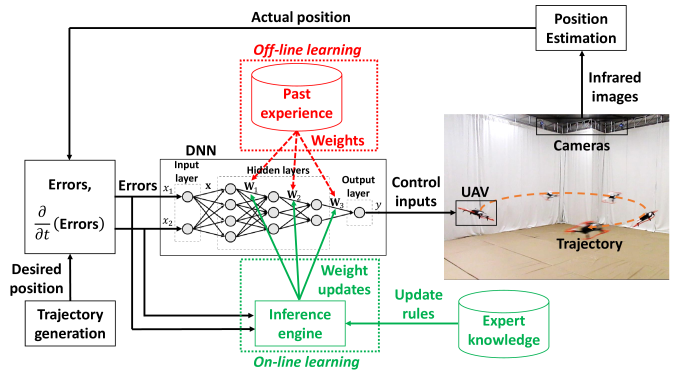
\includegraphics[width=0.7\linewidth]{Images/DNNcontroller}
	\caption{Illustration of how DNN controllers are replacing conventional controllers. The DNN is trained offline using input-output data obtained from different trajectories from a conventional controller. The DNN is shown to perform better than a conventional controller during real-time analysis for decision making by  Sarabakha et al. ~\cite{sarabakha2019online}.}
	\label{fig:dnncontroller}
\end{figure}

\begin{figure}
	\centering
	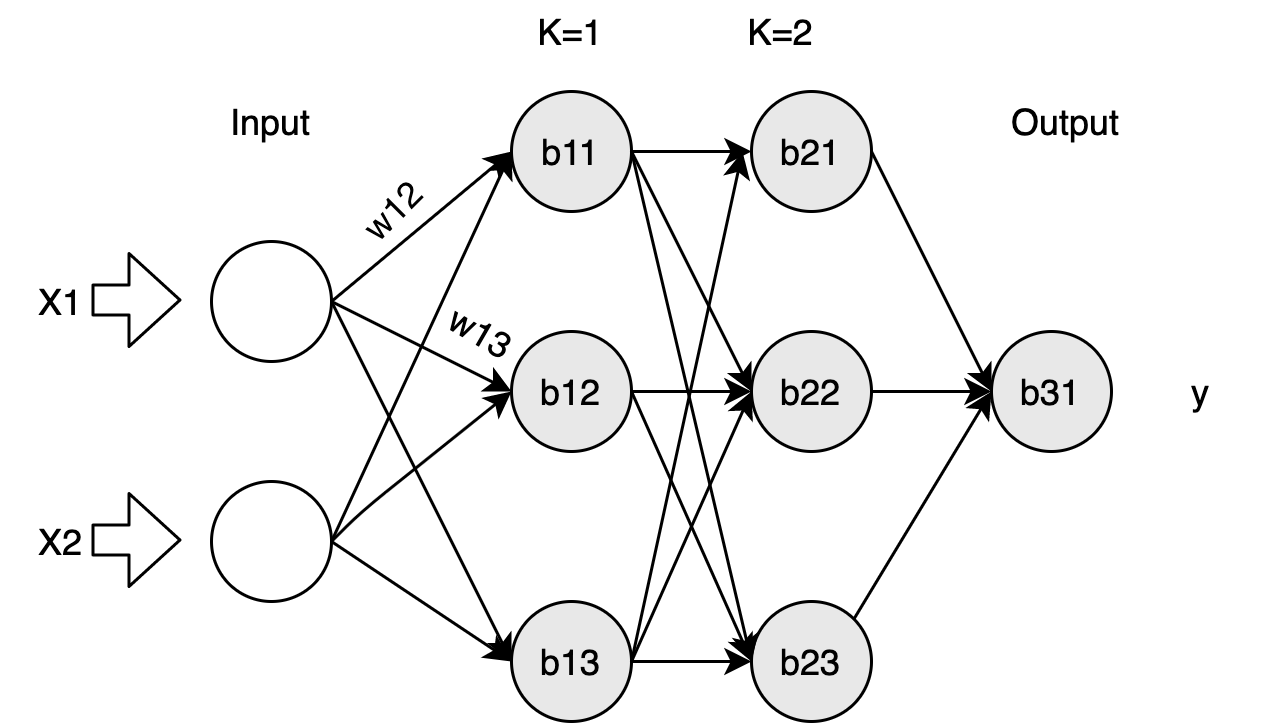
\includegraphics[width=0.7\linewidth]{Images/DNNstructure}
	\caption[DNN structure]{DNN controller structure with two hidden layers K=1,2, two inputs x1 and x2 and one output y. This is an example of a fully connected network.}
	\label{fig:dnn-controller}
\end{figure}

\section{Modeling Mixed-Integer Linear Programming Problems}
\label{milp}
We present a general structure that is required for building a \ac{LP} model, specifically a \ac{MILP} model.
\ac{MILP} is a \ac{LP} where some of the variables are restricted to be integers. 
We introduce the notion of \ac{MILP} because we use the underlying techniques to model \ac{DNN}s, and systematically reason about them in different scenarios with minimal effort. 
An \ac{LP} is characterized by the following components. 

\begin{enumerate}
	\item A \ac{LP} contains a set of decision variables, which are the unknown quantities or decisions that are to be optimized. 
	\item The function that assesses the quality of the solution is called an objective function or the cost function.
	\item \ac{LP}'s goal is to minimize or maximize the value of an objective function. 
	The decisions that are to be made depends on the requirements and restrictions of the  system modeled as \ac{LP}.
	\item A solution that satisfies all constraints is called a feasible solution. 
	Feasible solutions that achieve the best cost function value are called as optimal solutions. 
\end{enumerate}


The general form of a \ac{LP}  is shown in Equations 2.1. 
Values of $c$ denote the objective coefficient. 
$x_i$ denotes decision variables.
$b_i$ denotes the constraints.
As this is a linear model, so non-linear terms, for instance, multiplication of $z$ variables, are not allowed. 

\begin{equation}
\begin{aligned}
& \underset{x}{\text{min/max}}
& & c^T x \\
& \text{subject to} & &  Ax \leq b_i \\
& & &  \sum_{i=1}^{n} x_i =1 \\
& & &  x_j, \; \forall j \in N. \\
\end{aligned}
\end{equation}


We simplify the \ac{DNN} by modeling it as a \ac{MILP} which we will elaborate more in Chapter ~\ref{evaluation}.  

There are multiple tools that build \ac{MILP} models such as Cplex ~\cite{cplex}, and Gurobi ~\cite{gurobi}.
Both are widely used tools; however, we choose Gurobi for our work due to its more intuitive interface and python support.



\section{Problem Statement}
\label{problemstatement}

Given a trained DNN with fixed parameters our goal is to understand if the  \ac*{RFDIA} in classical control theory can also be applied to a \ac{DNN}.
This leads to two sub-problems as follows.

\begin{problem}
	How can we identify the critical inputs i.e inputs that  affect the final outputs the most on being perturbed in a \ac{DNN}?
\end{problem}

\begin{problem}
	What is the smallest perturbation to the critical input(s) that can produce \ac{RFDIA}?
\end{problem}




